\section{Матричный калькулятор}

\textbf{Задание:} Создать приложение, реализующее основные операции с векторами и матрицами:

\begin{enumerate}
    \item Ввод матрицы, вектора
    \item Создание матриц (единичная, матрица как набор векторов)
    \item Умножение на число, вектор, матрицу
    \item Сложение/вычитание двух матриц
    \item Сложение/вычитание двух векторов
    \item Скалярное и векторное произведение двух векторов
    \item Транспонированная матрица
    \item Определитель, ранг матрицы
\end{enumerate}
Выводить сообщения об ошибках (ввод не числа, несоответствие размерностей)

Интерфейс приложения можно условно разделить на четыре части, две из которых
отвечают за определение соответствующих аргументов операции, третья
за непосредственно саму операцию, а четвертая графически отображает
аргументы и результат

Вид окна представлен на рисунке \ref{fig:task6_form}.
\begin{figure}[H]
    \centering
    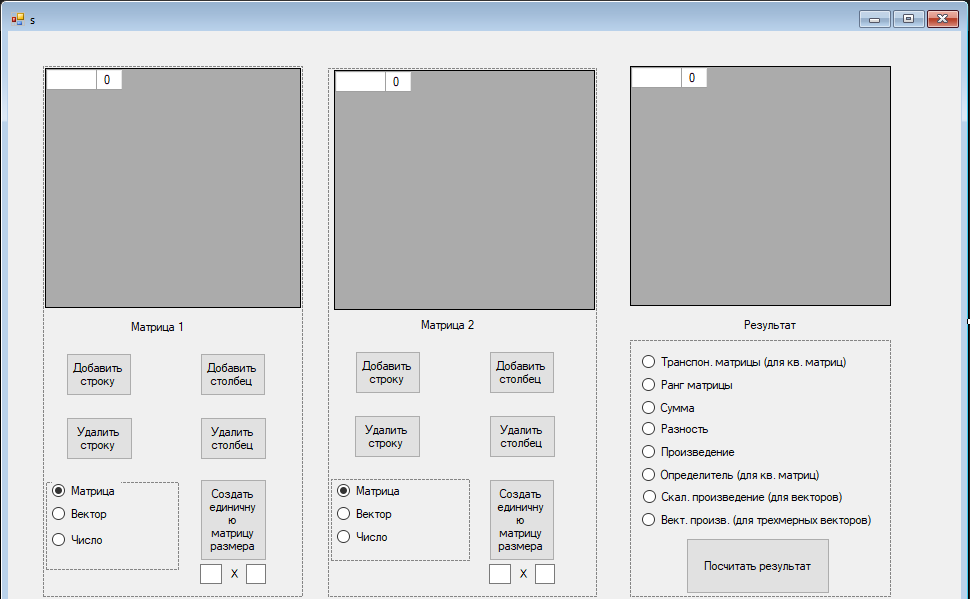
\includegraphics[scale=0.7]{task6/form.png}
    \caption{Внешний вид формы программы}
    \label{fig:task6_form}
\end{figure}

У элементов изменены значения некоторых атрибутов. 
Значения измененных атрибутов представлены в таблице \ref{table:params6}.

\begin{longtable}{|l|l|}
    Наименование атрибута & Значение\cr\hline
    \multicolumn{2}{|l|}{Для формы}\cr\hline
    \verb"Text" & \verb"Браузер "Амиго""\cr\hline
    \verb"FormBorderStyle" & \verb"FixedSingle"\cr\hline
    \verb"MaximizeBox" & \verb"False"\cr\hline
    \multicolumn{2}{|l|}{Для первой группы}\cr\hline
    \verb"(Name)" & \verb"MatrixGroup1"\cr\hline
    \multicolumn{2}{|l|}{Для второй группы}\cr\hline
    \verb"(Name)" & \verb"MatrixGroup2"\cr\hline
    \multicolumn{2}{|l|}{Для третьей группы}\cr\hline
    \verb"(Name)" & \verb"Result_Group"\cr\hline
    \multicolumn{2}{|l|}{Для надписи первой матрицы}\cr\hline
    \verb"(Name)" & \verb"initLabel"\cr\hline
    \verb"Text" & \verb"Матрица 1"\cr\hline
    \multicolumn{2}{|l|}{Для надписи второй матрицы}\cr\hline
    \verb"(Name)" & \verb"xLabel"\cr\hline
    \verb"Text" & \verb"Матрица 2"\cr\hline
    \multicolumn{2}{|l|}{Для третьей надписи}\cr\hline
    \verb"(Name)" & \verb"resultLabel"\cr\hline
    \verb"Text" & \verb"Результат"\cr\hline
    \multicolumn{2}{|l|}{Для радиокнопки "Матрица" для группы 1}\cr\hline
    \verb"(Name)" & \verb"Grid1_MatrixRBtn"\cr\hline
    \verb"Text" & \verb"Матрица"\cr\hline
    \multicolumn{2}{|l|}{Для радиокнопки "Вектор" для группы 1}\cr\hline
    \verb"(Name)" & \verb"Grid1_VectorRBtn"\cr\hline
    \verb"Text" & \verb"Вектор"\cr\hline
    \multicolumn{2}{|l|}{Для радиокнопки "Число" для группы 1}\cr\hline
    \verb"(Name)" & \verb"Grid1_NumRBtn"\cr\hline
    \verb"Text" & \verb"Число"\cr\hline
    \multicolumn{2}{|l|}{Для радиокнопки "Матрица" для группы 2}\cr\hline
    \verb"(Name)" & \verb"Grid2_MatrixRBtn"\cr\hline
    \verb"Text" & \verb"Матрица"\cr\hline
    \multicolumn{2}{|l|}{Для радиокнопки "Вектор" для группы 2}\cr\hline
    \verb"(Name)" & \verb"Grid2_VectorRBtn"\cr\hline
    \verb"Text" & \verb"Вектор"\cr\hline
    \multicolumn{2}{|l|}{Для радиокнопки "Число" для группы 2}\cr\hline
    \verb"(Name)" & \verb"Grid2_NumRBtn"\cr\hline
    \verb"Text" & \verb"Число"\cr\hline
    \multicolumn{2}{|l|}{Для радиокнопки транспонирования для группы 3}\cr\hline
    \verb"(Name)" & \verb"Transposition_RBtn"\cr\hline
    \verb"Text" & \verb"Транспон. матрицы (для кв. матриц)"\cr\hline
    \multicolumn{2}{|l|}{Для радиокнопки ранга матрицы для группы 3}\cr\hline
    \verb"(Name)" & \verb"Rank_RBtn"\cr\hline
    \verb"Text" & \verb"Ранг матрицы"\cr\hline
    \multicolumn{2}{|l|}{Для радиокнопки суммы для группы 3}\cr\hline
    \verb"(Name)" & \verb"Sum_RBtn"\cr\hline
    \verb"Text" & \verb"Сумма"\cr\hline
    \multicolumn{2}{|l|}{Для радиокнопки разности для группы 3}\cr\hline
    \verb"(Name)" & \verb"Difference_RBtn"\cr\hline
    \verb"Text" & \verb"Разность"\cr\hline
    \multicolumn{2}{|l|}{Для радиокнопки произведения для группы 3}\cr\hline
    \verb"(Name)" & \verb"Mult_RBtn"\cr\hline
    \verb"Text" & \verb"Произведение"\cr\hline
    \multicolumn{2}{|l|}{Для радиокнопки определителя для группы 3}\cr\hline
    \verb"(Name)" & \verb"Det_RBtn"\cr\hline
    \verb"Text" & \verb"Определитель (для кв. матриц) "\cr\hline
    \multicolumn{2}{|l|}{Для радиокнопки скалярного произведения для группы 3}\cr\hline
    \verb"(Name)" & \verb"ScalarMultiply_RBtn"\cr\hline
    \verb"Text" & \verb"Скалярное произведение (для векторов) "\cr\hline
    \multicolumn{2}{|l|}{Для радиокнопки векторного произведения для группы 3}\cr\hline
    \verb"(Name)" & \verb"VectorMultiply_RBtn"\cr\hline
    \verb"Text" & \verb"Векторное произведение (для трехмерных векторов)"\cr\hline
    \multicolumn{2}{|l|}{Для кнопки создания единичной матрицы для группы 1}\cr\hline
    \verb"(Name)" & \verb"CreateMatrix1_Btn"\cr\hline
    \verb"Text" & \verb"Создать единичную матрицу размера"\cr\hline
    \multicolumn{2}{|l|}{Для кнопки создания единичной матрицы для группы 2}\cr\hline
    \verb"(Name)" & \verb"CreateMatrix2_Btn"\cr\hline
    \verb"Text" & \verb"Создать единичную матрицу размера"\cr\hline
    \multicolumn{2}{|l|}{Для знака размерности для группы 1}\cr\hline
    \verb"(Name)" & \verb"Scale_label1"\cr\hline
    \verb"Text" & \verb"X"\cr\hline
    \multicolumn{2}{|l|}{Для знака размерности для группы 2}\cr\hline
    \verb"(Name)" & \verb"Scale_label2"\cr\hline
    \verb"Text" & \verb"X"\cr\hline
    \multicolumn{2}{|l|}{Для текстового поля N размерности для группы 1}\cr\hline
    \verb"(Name)" & \verb"N1_TextBox"\cr\hline
    \multicolumn{2}{|l|}{Для текстового поля M размерности для группы 1}\cr\hline
    \verb"(Name)" & \verb"M1_TextBox"\cr\hline
    \multicolumn{2}{|l|}{Для текстового поля N размерности для группы 2}\cr\hline
    \verb"(Name)" & \verb"N2_TextBox"\cr\hline
    \multicolumn{2}{|l|}{Для текстового поля M размерности для группы 2}\cr\hline
    \verb"(Name)" & \verb"M2_TextBox"\cr\hline

    \multicolumn{2}{|l|}{Для кнопки "Добавить строку" для группы 1}\cr\hline
    \verb"(Name)" & \verb"Grid1_btnAddRow"\cr\hline
    \verb"Text" & \verb"Добавить строку"\cr\hline
    \multicolumn{2}{|l|}{Для кнопки "Добавить столбец" для группы 1}\cr\hline
    \verb"(Name)" & \verb"Grid1_btnAddColumn"\cr\hline
    \verb"Text" & \verb"Добавить столбец"\cr\hline
    \multicolumn{2}{|l|}{Для кнопки "Удалить строку" для группы 1}\cr\hline
    \verb"(Name)" & \verb"Grid1_btnRmvRow"\cr\hline
    \verb"Text" & \verb"Удалить строку"\cr\hline
    \multicolumn{2}{|l|}{Для кнопки "Удалить столбец" для группы 1}\cr\hline
    \verb"(Name)" & \verb"Grid1_btnRmvColumn"\cr\hline
    \verb"Text" & \verb"Удалить столбец"\cr\hline
    \multicolumn{2}{|l|}{Для кнопки "Добавить строку" для группы 2}\cr\hline
    \verb"(Name)" & \verb"Grid2_btnAddRow"\cr\hline
    \verb"Text" & \verb"Добавить строку"\cr\hline
    \multicolumn{2}{|l|}{Для кнопки "Добавить столбец" для группы 2}\cr\hline
    \verb"(Name)" & \verb"Grid2_btnAddColumn"\cr\hline
    \verb"Text" & \verb"Добавить столбец"\cr\hline
    \multicolumn{2}{|l|}{Для кнопки "Удалить строку" для группы 2}\cr\hline
    \verb"(Name)" & \verb"Grid2_btnRmvRow"\cr\hline
    \verb"Text" & \verb"Удалить строку"\cr\hline
    \multicolumn{2}{|l|}{Для кнопки "Удалить столбец" для группы 2}\cr\hline
    \verb"(Name)" & \verb"Grid2_btnRmvColumn"\cr\hline
    \verb"Text" & \verb"Удалить столбец"\cr\hline
    \multicolumn{2}{|l|}{Для кнопки добавления ряда}\cr\hline
    \verb"(Name)" & \verb"btnAddRow"\cr\hline
    \verb"Text" & \verb"Добавить"\cr\hline
    \multicolumn{2}{|l|}{Для кнопки удаления ряда}\cr\hline
    \verb"(Name)" & \verb"btnRemoveRow"\cr\hline
    \verb"Text" & \verb"Удалить"\cr\hline
    \multicolumn{2}{|l|}{Для кнопки добавления столбца}\cr\hline
    \verb"(Name)" & \verb"btnAddColumn"\cr\hline
    \verb"Text" & \verb"Добавить"\cr\hline
    \multicolumn{2}{|l|}{Для кнопки удаления столбца}\cr\hline
    \verb"(Name)" & \verb"btnRemoveColumn"\cr\hline
    \verb"Text" & \verb"Удалить"\cr\hline
    \multicolumn{2}{|l|}{Для обработчика ошибок}\cr\hline
    \verb"(Name)" & \verb"errorProvider1"\cr\hline

    \caption{Значения атрибутов элементов в приложении <<Матричный калькулятор}
    \label{table:params6}
\end{longtable}

Программа работает за счет дополнительно написанной библиотеки для работы с матрицами 
с помощью \verb|std::vector| библиотеки STL. В ней реализованы все операции.

Полный код библиотеки приведен в приложении B.

Кроме того, написаны две вспомогательный функции, представляющие из себя связки
между \verb|std::vector| и \verb|DataGridView|. Код приведен ниже:

\inputminted[fontsize=\small, breaklines=true, style=bw, linenos, encoding=cp1251, outencoding=utf8]{cpp}{task6/Misc.h}

Примеры работы приведены ниже:

\begin{figure}[H]
    \centering
    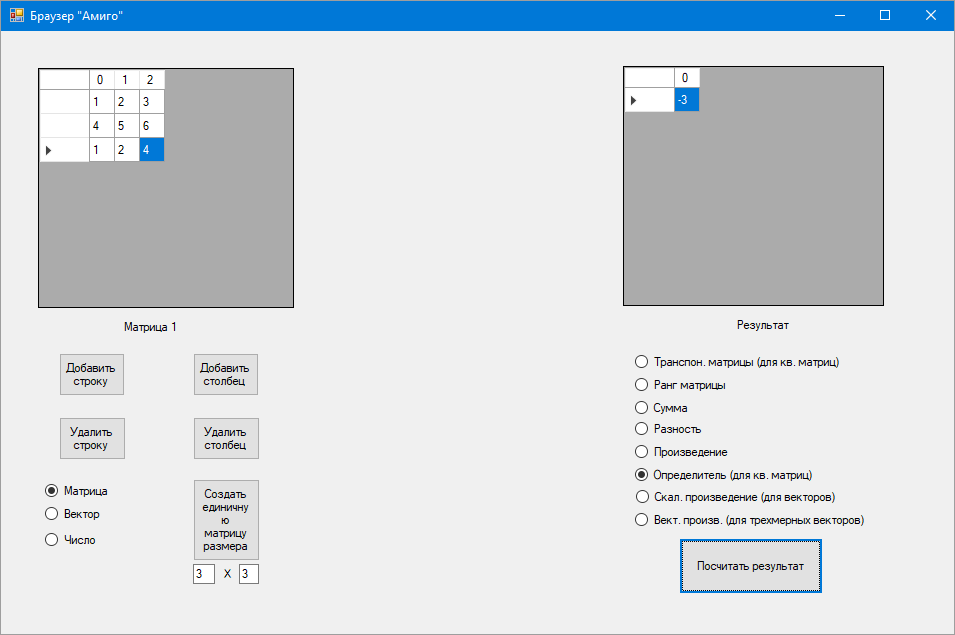
\includegraphics[scale=0.4]{task6/det.png}
    \caption{Пример нахождения определителя матрицы}
\end{figure}

\begin{figure}[H]
    \centering
    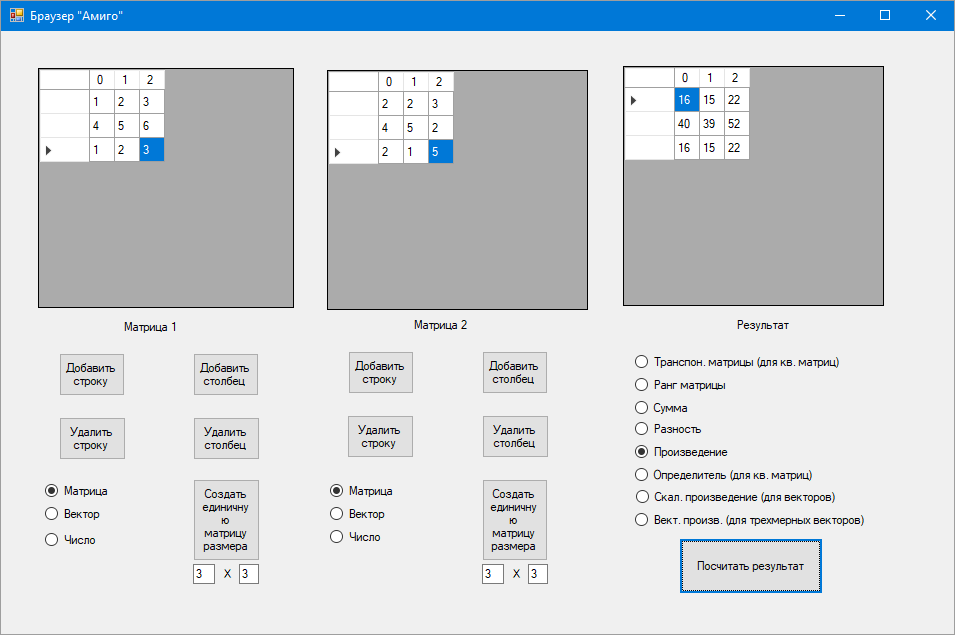
\includegraphics[scale=0.4]{task6/mult.png}   
    \caption{Пример нахождения векторного произведения}
\end{figure}

\begin{figure}[H]
    \centering
    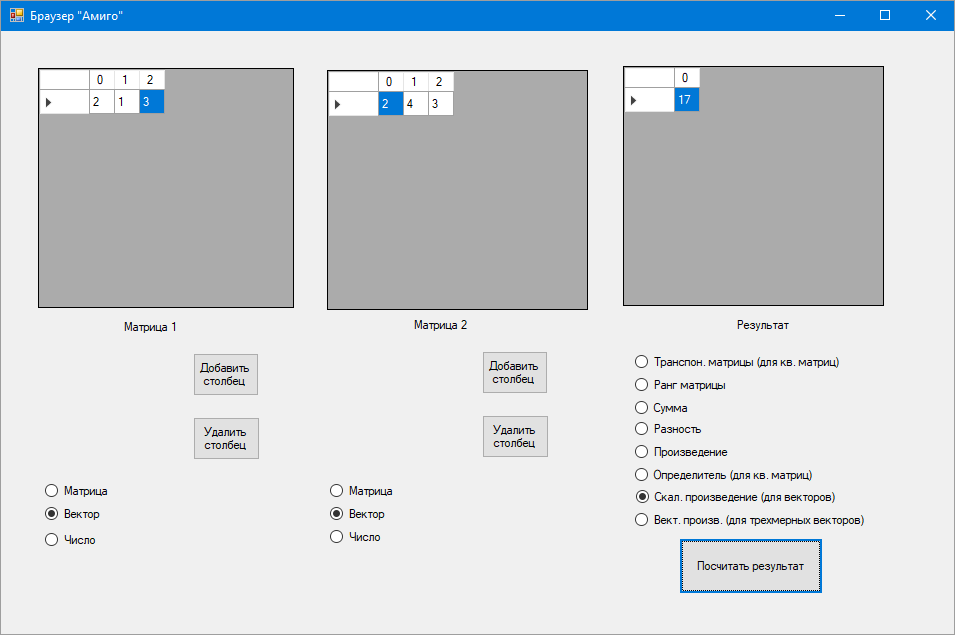
\includegraphics[scale=0.4]{task6/scalar.png}
    \caption{Пример нахождения скалярного произведения векторов}
\end{figure}

Можно заметить, что интерфейс приложения динамически изменяется в 
зависимости от выбранных параметров в соответствующих радиокнопках.

Контроль за корректностью введенных данных осуществляется внутри соответствующих
функций. 

В случае, если вводятся некорректные данные или операция не поддерживается
над операндами этого типа "--- будет выведено сообщение об ошибке:
\begin{figure}[H]
    \centering
    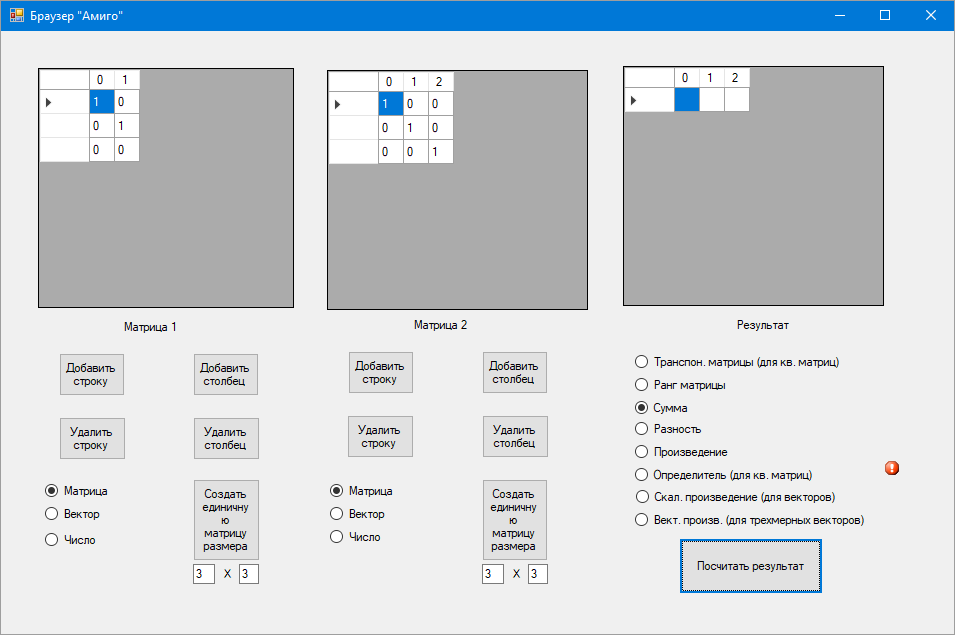
\includegraphics[scale=0.4]{task6/error1.png}
    \caption{Пример обработки ошибки}
\end{figure}
Полный код программы приведен в приложении А.

